\begin{figure}[h]
\centering
\textbf{Class River}

\begin{tabular}{|p{0.4\linewidth}p{0.4\linewidth}|}
\hline & \\
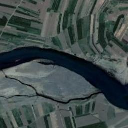
\includegraphics[width=\linewidth,frame]{figures/examples_assests/linear_probing/river_1.pdf} &
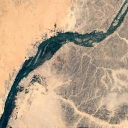
\includegraphics[width=\linewidth,frame]{figures/examples_assests/linear_probing/river_2.pdf} \\
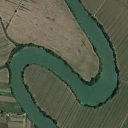
\includegraphics[width=\linewidth,frame]{figures/examples_assests/linear_probing/river_3.pdf} & 
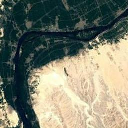
\includegraphics[width=\linewidth,frame]{figures/examples_assests/linear_probing/river_4.pdf} \\
\hline
\end{tabular}
\\
\textbf{Class Industrial Area}
\\
\begin{tabular}{|p{0.4\linewidth}p{0.4\linewidth}|}
\hline & \\
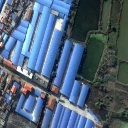
\includegraphics[width=\linewidth,frame]{figures/examples_assests/linear_probing/industry_1.pdf} &
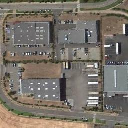
\includegraphics[width=\linewidth,frame]{figures/examples_assests/linear_probing/industry_2.pdf} \\
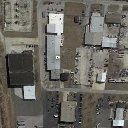
\includegraphics[width=\linewidth,frame]{figures/examples_assests/linear_probing/industry_3.pdf} & 
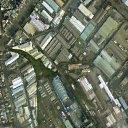
\includegraphics[width=\linewidth,frame]{figures/examples_assests/linear_probing/industry_4.pdf}\\
\hline
\end{tabular}
\caption{\textbf{Linear Probing (Classification) example from \emph{RESISC45}.}}
\label{fig:linear_example}
\end{figure}